\section{Siamese Multi-Object Tracking Framework}
\label{sec:SiamMOT}

% ##############################################################################
\subsection{Motivation For Model and Dataset Selection}

Our initial motivation to adopt the \gls{siammot}~\cite{shuai2021siammot} tracker as the base for our custom implementation was that it exploited the best practices honed within the \gls{sot} community and that it had been published very recently, reaping a \gls{sota} performance back then. Besides, we saw several potential parts for improvement, namely its ability to inherently handle trivial cases of short-term occlusion during the identity association stage. Even though we were above all concerned with Siamese \gls{sot}, we also knew that traffic analysis is inherently preoccupied with multiple objects. But still, we tried to avoid \gls{mot} at the beginning as it introduced additional problems to overcome.

However, training, as well as evaluation of the developed tracker, requires a lot of annotated data. Admittedly, we devoted a great deal of time to finding datasets for tracking single vehicles, but to no avail. Nevertheless, the \interreg{} project provided a lot of data that involved traffic scenes. We mentioned this project as part of our discussion related to homography ranking (\chaptertext{}~\ref{chap:HomographyRanking} on page \pageref{chap:HomographyRanking}). The major drawback is that the data encompass only a limited view of the road (\figtext{}~\ref{fig:InterregDatasetSample}).

Consequently, we set out to search for different datasets, preferably with a target use of benchmarking tracking algorithms. And we found the \uadetrac{} dataset (\sectiontext{}~\ref{ssec:DatasetUADETRAC} on page \pageref{ssec:DatasetUADETRAC}), which we consider one of the best available datasets. The data fit the task of traffic analysis using a static camera under various conditions very well. However, one needs to officially ask for the data annotations. We were unfortunate enough that the public web dedicated to this benchmark was broken for a long time and we had to personally negotiate with the authors to provide unofficial access to the data.

% ------------------------------------------------------------------------------
\begin{figure}[!t]
    \centering
    \begin{subfigure}[b]{0.4\textwidth}
        \centering
        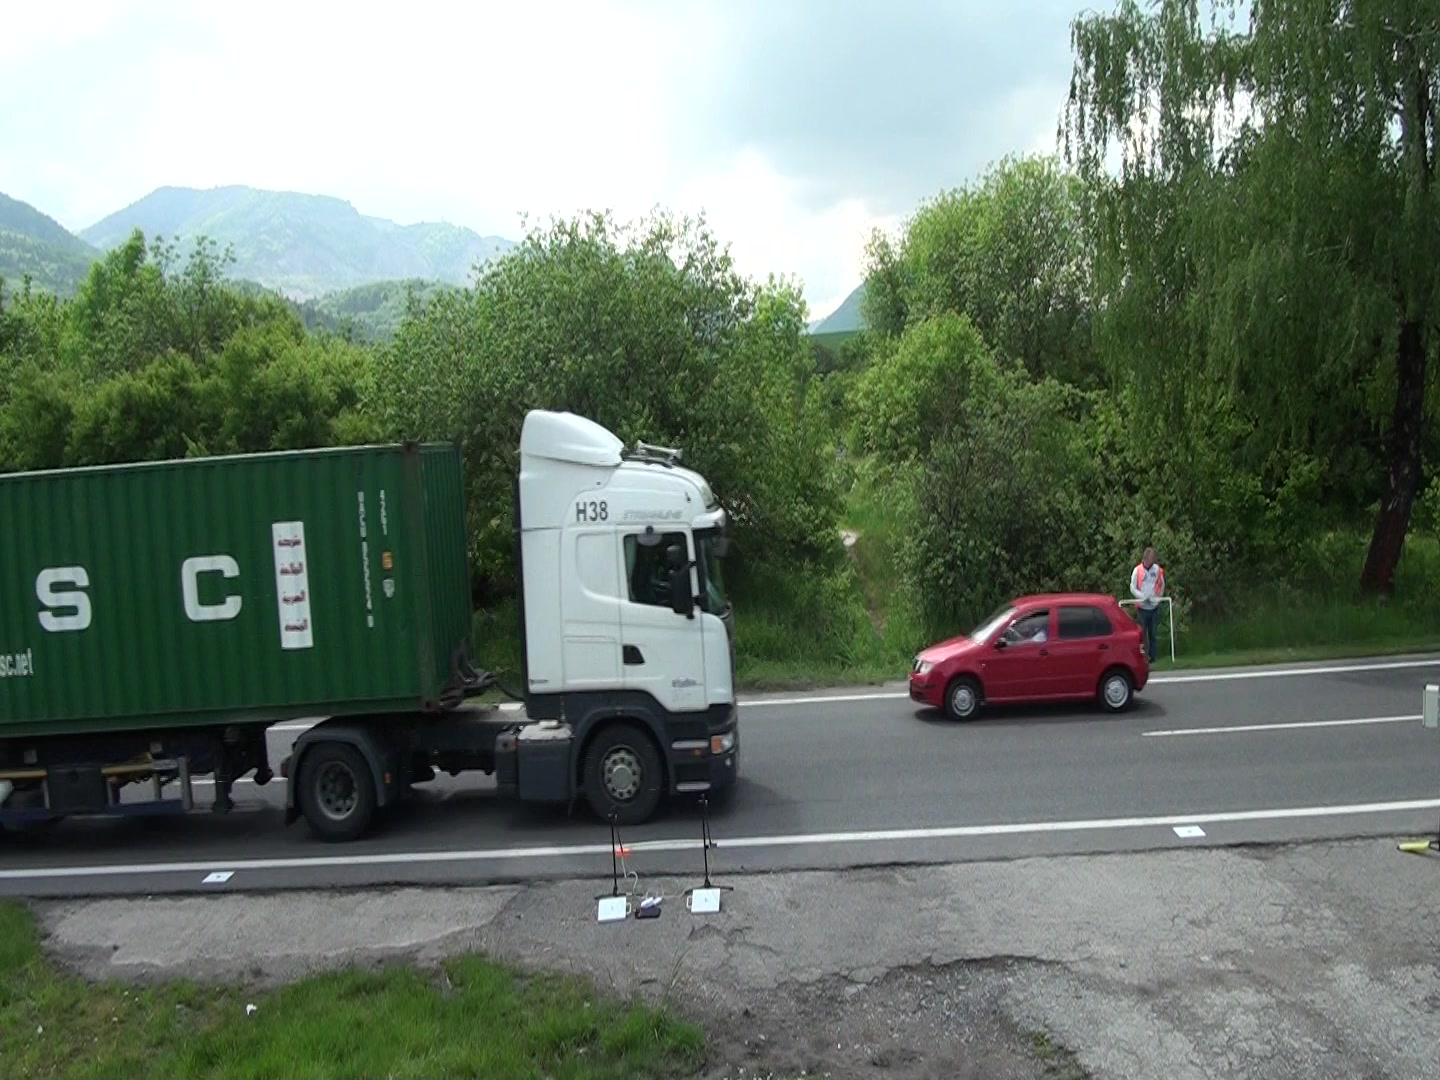
\includegraphics[width=\textwidth]{figures/siamese_tracking/interreg_sample_01.jpg}
        \caption[]{}
    \end{subfigure}
    \begin{subfigure}[b]{0.4\textwidth}
        \centering
        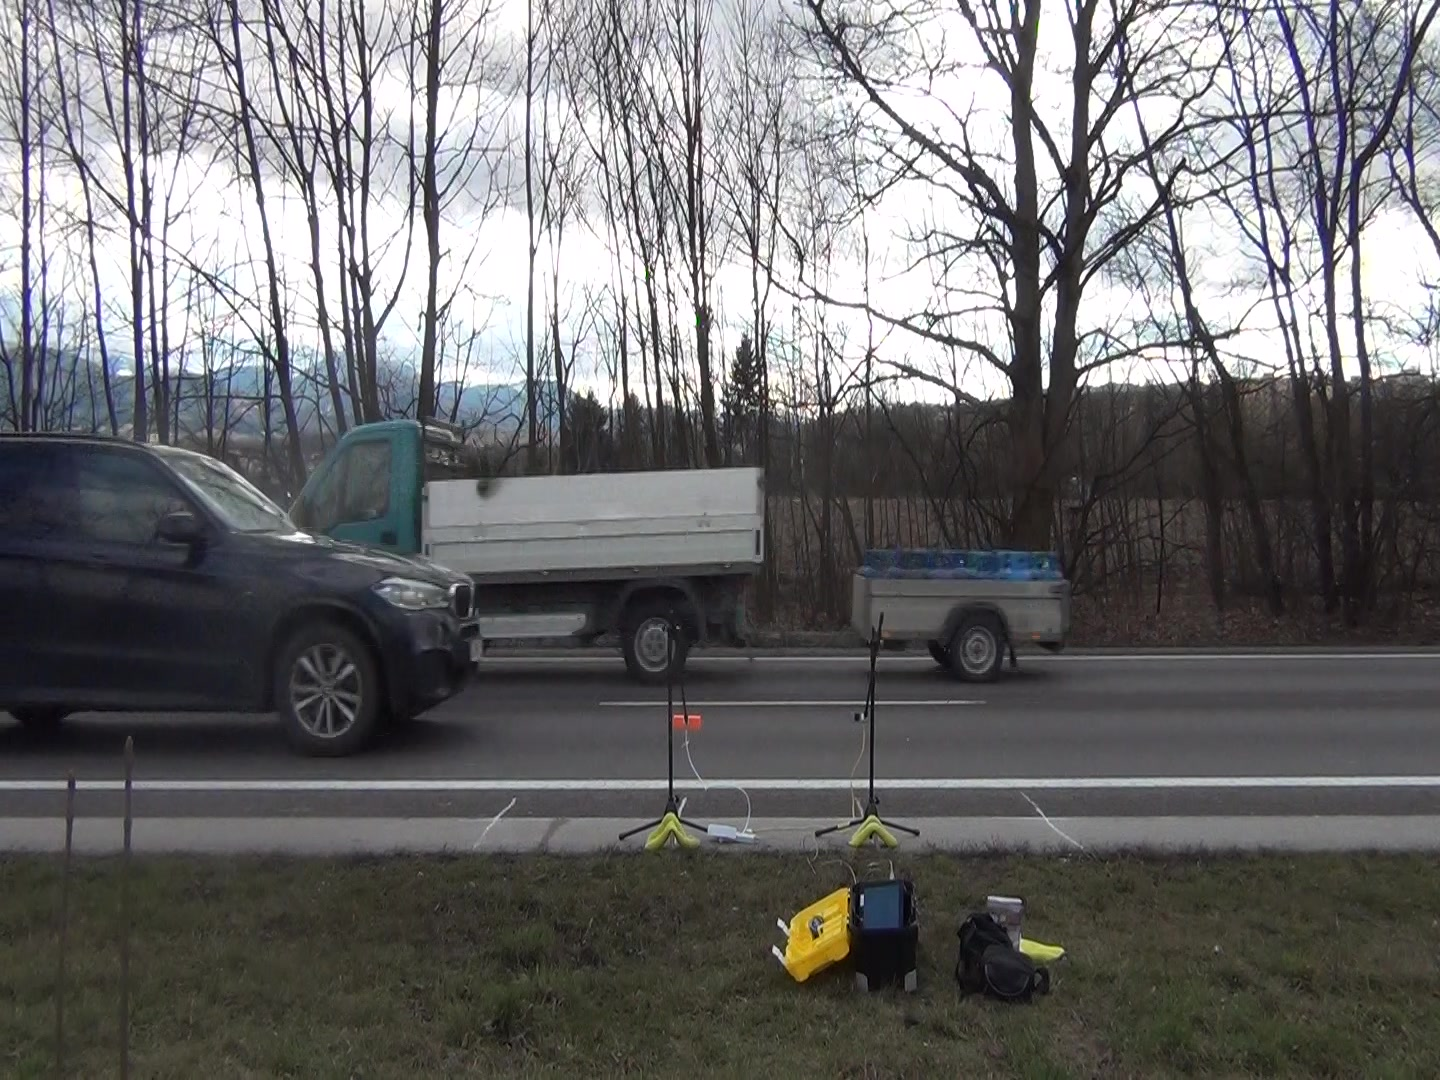
\includegraphics[width=\textwidth]{figures/siamese_tracking/interreg_sample_02.jpg}
        \caption[]{}
    \end{subfigure}
    \caption[Interreg dataset sample]{Road scenes we encountered when working on the \interreg{} project.}
    \label{fig:InterregDatasetSample}
\end{figure}

% ------------------------------------------------------------------------------

% ##############################################################################
\subsection{General Description}

The authors of~\cite{shuai2021siammot} tracker focused on improving online \gls{mot}. As far as their methodology was concerned, they employed a region-based approach~\cite{ren2017fasterrcnn} in conjunction with a Siamese multiple-object tracking network, hence the name \gls{siammot}. Broadly speaking, this architecture employs a Siamese tracker for motion estimation between two frames. We would like to note that all the principles so far discussed regarding Siamese trackers apply here. However, as already suggested, the adoption of \gls{rpn} enables this framework to have more information available. Not only there is the motion prediction from the Siamese tracker, but there are also detections produced by a \gls{fasterrcnn} object detector~\cite{ren2017fasterrcnn} that is integrated within the whole architecture. Subsequently, an online solver is utilized to merge the predictions obtained from the tracker and detector heads.

We will dissect this framework in great detail since we have studied it scrupulously. We performed multiple experiments, many of which did not yield expected improvements. Nevertheless, the practical part of our work was focused on contributing to the open-source repository dedicated to this project developed by several Amazon researchers~\cite{websiammotoriggithub}. We followed a standard path of how contributing to open source projects should be done in a transparent and, more importantly, compatible fashion. We initialized a fresh fork of this project on our personal GitHub account~\cite{websiammotforkgithub} to preserve as much compatibility with the original software as possible and not to strip ourselves of the opportunity to easily receive potential updates from the original repository.

During our development, we often engaged in discussions related to this project incentivized by other researchers who were also working on the very same codebase and trying to either only apply this work to their specific use case or even extend the model. Our detailed knowledge of this model acquired through deliberate work on this project often helped several other programmers who dealt with various issues. From the programming standpoint, our work involved a considerable amount of programming, even though the base architecture was provided and was fully functional from the start, even though the initial setup lasted for several days as well, mainly due to libraries support and compatibility issues. We would like to emphasize that the project consisted of several thousand lines of source code programmed purely in Python programming language. Concerning the deep learning aspect, the \pytorch{} library~\cite{paszke2019pytorch} was primarily used. It is a widely known library aimed at building deep neural network models while exploiting automatic differentiation.

% ##############################################################################
\subsection{Model Architecture}

The two key aspects of the the \gls{siammot} architecture are \gls{fasterrcnn}~\cite{ren2017fasterrcnn} object detector and Siamese tracker. The salient element of the \gls{fasterrcnn} is the \gls{rpn}. Simply put, \gls{siammot} adds a region-based Siamese tracker along the standard $2$-stage object detection pipeline in order to model instance-level motion.

As depicted in \figtext{}~\ref{fig:SiamMOTArchitecture}, the input consists of two frames, namely $\mtxsup{I}{t}$ and $\mtxsup{I}{t + \delta}$, accompanied by a set of detected object instances $\mtxsup{R}{t} = \cbrackets{\subsup{R}{1}{t}, \subsup{R}{2}{t}, \dots, \subsup{R}{i}{t}, \dots}$ at time $t$. During inference, the detection head produces a set of detected object instances $\mtxsup{R}{t + \delta}$ whilst the tracker's task is to propage the detections $\mtxsup{R}{t}$ to time $t + \delta$, and yielding the tracker output denoted as $\mtxsup{\tilde{R}}{t + \delta}$. Please note that it is not the output of the entire tracker, only of the Siamese tracker itself. These instances have to be further processed.

This framework relies on a motion model that tracks each detected object instance from time $t$ to $t + \delta$. A specific \gls{bbox} $\subsup{R}{i}{t}$ at time $t$ is propagated to its future counterpart $\subsup{\tilde{R}}{i}{t + \delta}$ at time $t + \delta$. This process is then completed by a spatial matching phase the objective of which is the associaton of the tracker output $\subsup{\tilde{R}}{i}{t + \delta}$ with detections $\subsup{R}{i}{t + \delta}$ at time $t + \delta$ such that detected instances are linked from $t$ to $t + \delta$.

Assume there is a specific object instance $i$ detected at time $t$. Then, the Siamese tracker searches for this particular instance at frame $\mtxsup{I}{t + \delta}$ while exploiting a contextual window spanning a fixed neighborhood of the object's location (\ietext{}, $\subsup{R}{i}{t}$) at frame $\mtxsup{I}{t}$. In order to define this step more formally, consider the following dependency:
\begin{equation}
    \label{eq:SiamMOTSiameseTracker}
    \rbrackets{
        \subsup{v}{i}{t + \delta},
        \subsup{\tilde{R}}{i}{t + \delta}
    } =
    \func{\mathcal{T}}{
        \mtxsubsup{f}{R_i}{t}, \mtxsubsup{f}{S_i}{t + \delta}; \Theta
    },
\end{equation}
where $\mathcal{T}$ is a module (head) represented by the Siamese tracker with learnable parameters $\Theta$. In light of the already stated efficiency of this framework in terms reusing information as much as possible, the module $\mathcal{T}$ is trained on shared feature maps extracted from the backbone using \gls{roi}-align operations. As a short reminder, a basic Siamese tracker uses an exemplar image encoded as a kernel to search for the occurrence of the corresponding object in a future frames over a specific search region that should be, by definition, greater than the exemplar region. Thus, the feature map $\mtxsubsup{f}{R_i}{t}$ is extracted over the region $\subsup{R}{i}{t}$ contained in the frame $\mtxsup{I}{t}$. Analogically, the feature map $\mtxsubsup{f}{S_i}{t + \delta}$ is extracted over the search region $\subsup{S}{i}{t + \delta}$ delineated in the frame $\mtxsup{I}{t + \delta}$. The region $\subsup{S}{i}{t + \delta}$ is computed by simple expansion of the region $\subsup{R}{i}{t}$ by a factor $r$, such that $r > 1$, while preserving the location of the geometric center, as illustrated in \figtext{}~\ref{fig:SiamMOTArchitecture} by the dashed \gls{bbox}. Last but not least, $\subsup{v}{i}{t + \delta}$ represents the visibility confidence for the detected instance $i$ at time $t + \delta$. This visibility score reflects the tracker's prediction confidence, and so the value $\subsup{v}{i}{t + \delta}$ should be high if the instance is visible in $\subsup{S}{i}{t + \delta}$, otherwise the value should be low. On top of this formulation that is reminiscent of single object tracking, in the \gls{mot} context \eqtext{}~\ref{eq:SiamMOTSiameseTracker} is applied multiple times, \ietext{}, for each object detected in frame $t$, signified by $\subsup{R}{i}{t} \in \mtxsup{R}{t}$. However, from implementation's perspective, all these operations can run in parallel and thus the backbone features are computed only once.

% ------------------------------------------------------------------------------
\begin{figure}[t]
    \centering
    \includegraphics[width=\linewidth]{figures/siamese_tracking/siammot_architecture.pdf}
    \caption[\gls{siammot} architecture]{The \gls{siammot} tracker that detects and associates object instances simultaneously. The Siamese tracker in the top branch serves the purpose of predicting the motion of objects, thus facilitating the temporal linking of objects in an online fashion. Simply put, the Siamese tracker module can be thought of as a single object tracker with all the pros and cons we have discussed so far. On the other hand, a $2$-stage object detection is performed as part of the bottom branch. These two branches are then merged using a solver that spatially and temporally attempts to match tracker and detector predictions to produce the tracker output. Note that the feature map corresponding to the frame $\mtxsup{I}{t}$ is shrunk to $\nicefrac{1}{2}$ of its actual size to fit the figure. Backbone features are identical in terms of tensor shapes for both inputs. \externalsrc{\cite{shuai2021siammot}}}
    \label{fig:SiamMOTArchitecture}
\end{figure}
% ------------------------------------------------------------------------------

The authors conjectured that motion modeling is of paramount importance for online \gls{mot}. Given our experience in this field so far, we agree. The motion modeling is practically responsible for association between $\mtxsup{R}{t}$ and $\mtxsup{R}{t + \delta}$. Despite its efficacy, there are still issues to be addressed. The association fails due to the following reasons:
\begin{enumerate}
    \item if $\mtxsup{\tilde{R}}{t + \delta}$ does not match to the correct object instance in $\mtxsup{R}{t + \delta}$,
    \item or if $\subsup{v}{i}{t + \delta}$ is low (below a specific threshold) for a visible object at time $t + \delta$.
\end{enumerate}
To tackle the problems outlined above, the Siamese tracker exploits various \gls{sota} techniques developed in the single-object Siamese tracking community. We affirmatively approve of the authors' decisions, since we deliberately elaborated on multiple aspects that this tracker heavily relies upon in our survey on Siamese tracking~\cite{ondrasovic2021siamese}.

As far as the Siamese part of the \gls{siammot} is concerned, the authors dubbed their technique as ``explicit motion modeling''. They also worked with ``implicit motion modeling'', but that branch of experiments was neither sufficiently expanded in the paper nor it is of particular importance to our research due to its inferior performance.

\subsubsection{Explicit Motion Modeling}

The most fundamental aspect of Siamese trackers is the cross-correlation operator (\sectiontext{}~\ref{eq:SiameseCrossCorrelation} on page~\pageref{eq:SiameseCrossCorrelation}) to generate a $2$D response map. In \gls{siammot}, this operation correlates each location of the search feature map (belonging to the search region) $\mtxsubsup{f}{S_i}{t + \delta}$ with the exemplar feature map $\mtxsubsup{f}{R_i}{t}$ to produce a response map
\begin{equation}
    \mtxsub{r}{i} = \mtxsubsup{f}{S_i}{t + \delta} \star \mtxsubsup{f}{R_i}{t}.
\end{equation}
Therefore, each map $r_i$ captures a different aspect of similarity at every pixel.

Inspired by the \gls{fcos}~\cite{tian2019fcos} visual object detector, this tracker adopts fully convolutional network $\psi$ to facilitate instance detection using the response map $\mtxsub{r}{i}$. Besides, the so-called \emph{centerness} is also utilized in this architecture (discussed later). The network $\psi$ enables a prediction of a dense visibility confidence map $\mtxsub{v}{i}$. Every pixel of $\mtxsub{v}{i}$ is used as an indicator of the likelihood that this pixel falls within the location of the target object. Besides, a dense location map $\mtxsub{p}{i}$ is also predicted with the goal of encoding offsets from that particular location to the top-left and bottom right \gls{bbox} corners. Consequently, the instance region at $\rbrackets{x, y}$ can be derived by the transformation
\begin{equation}
    \func{\mathcal{R}}{\func{\mtx{p}}{x, y}} =
    \sbrackets{x - l, y - t, x + r, y + b},
\end{equation}
where $\func{\mtx{p}}{x, y} = \sbrackets{l, t, r, b}$, \ietext{}, individual corner offsets. This map is then decoded as
\begin{equation}
    \begin{aligned}
                            & \subsup{\tilde{R}}{i}{t + \delta} =
        \func{\mathcal{R}}{\func{\mtxsub{p}{i}}{x^*, y^*}}                                                                      \\
                            & \subsup{v}{i}{t + \delta} = \func{\mtxsub{v}{i}}{x^*, y^*}                                        \\
        \text{s. t. } \quad & \rbrackets{x^*, y^*} = \underset{x, y}{\argmax} \rbrackets{\mtxsub{v}{i} \odot \mtxsub{\eta}{i}},
    \end{aligned}
\end{equation}
in which $\odot$ symbolizes the element-wise multiplication, $\mtxsub{\eta}{i}$ incurs a non-negative penalty score throughout the entire candidate region computed as
\begin{equation}
    \func{\mtxsub{\eta}{i}}{x, y} =
    \lambda \mathcal{C} +
    \rbrackets{1 - \lambda} \func{\mathcal{S}}{
        \func{\mathcal{R}}{
            \func{\mtx{p}}{x, y}
        },
        \subsup{R}{i}{t}
    }.
\end{equation}
Here, the letter $\lambda$, such that $0 \leq \lambda \leq 1$, is a weighting coefficient, $\mathcal{C}$ is the cosine-window function with respect to the geometric center of the previous target location given by $\subsup{R}{i}{t}$, and $\mathcal{S}$ is a Gaussian function that is supposed to penalize the height-to-width ratio changes between candidate region $\func{\mtx{p}}{x, y}$ and $\subsup{R}{i}{t}$. The penalty map aims to discourage abrupt changes in target location between individual frames during the course of tracking. This technique is widely adopted in Siamese trackers (\figtext{}~\ref{fig:CosineWindow} on page \pageref{fig:CosineWindow}).

\subsubsection{Loss Function}

The loss function for this model consists of multiple parts and for its completeness it requires a triplet $\rbrackets{\subsup{R}{i}{t}, \subsup{S}{i}{t + \delta}, \subsup{R}{i}{t + \delta}}$. The following function is minimized during the training:
\begin{equation}
    \begin{aligned}
        \lossf =
         & \sum_{\forall \rbrackets{x, y}}
        \func{l_{focal}}{
            \func{\mtxsub{v}{i}}{
                x, y
            },
            \func{\mtxsubsup{v}{i}{*}}{
                x, y
            }
        } +                                \\
         & \sum_{\forall \rbrackets{x, y}}
        \mathbbm{1}
        \sbrackets{
            \func{\mtxsubsup{v}{i}{*}}{
                x, y
            } = 1
        }
        \rbrackets{
            \func{w}{x, y}
            \cdot
            \func{l_{reg}}{
                \func{\mtxsub{p}{i}}{x, y},
                \func{\mtxsubsup{p}{i}{*}}{x, y}
            }
        }
    \end{aligned}.
\end{equation}
In the expression above, the pairs $\rbrackets{x, y}$ enumerate all valid positions within the $\subsup{S}{i}{t + \delta}$ region. The loss function dedicated to regression task, \ietext{}, $l_{reg}$, is formulated as the \gls{iou} loss for regression~\cite{danelljan2019atom, yu2016unitbox}. To address the class-imbalance problem in an effective way, the focal loss for classification~\cite{lin2018focal} given by the term $l_{focal}$ is employed, too. All ground-truth values are marked by the $*$ character. So,
\begin{equation}
    \func{\mtxsubsup{v}{i}{*}}{x, y} =
    \begin{cases}
        \begin{aligned}
             & 1 & \text{if } \rbrackets{x, y} \text{ is within } \subsup{R}{i}{*, t + \delta} \\
             & 0 & \text{otherwise}                                                            \\
        \end{aligned}
    \end{cases},
\end{equation}
and
\begin{equation}
    \func{\mtxsubsup{p}{i}{*}}{x, y} =
    \sbrackets{
        x - \subsup{x}{0}{*},
        y - \subsup{y}{0}{*},
        \subsup{x}{1}{*} - x,
        \subsup{y}{1}{*} - y
    },
\end{equation}
where $\rbrackets{\subsup{x}{0}{*}, \subsup{y}{0}{*}}$ and $\rbrackets{\subsup{x}{1}{*}, \subsup{y}{1}{*}}$ correspond to the top-left and bottom-right coordinates of the ground-truth \gls{bbox} $\subsup{R}{i}{t + \delta}$, respectively. Following the line of inspiration from the \gls{fcos}~\cite{tian2019fcos} tracker, the regression loss $l_{reg}$ is additionally modulated by computing the \emph{centerness} for every location (\figtext{}~\ref{fig:FCOSCenterness}). This concept describes the amount of deviation of the pixel's location from the object center. The reason for adding this score was to suppress locations that are further away from the object's center, because they produced low-quality \gls{bbox} predictions. This score is then used as a weighting. The \emph{centerness} coefficient $\func{w}{x, y}$ is calculated for each pixel with respect to the target instance $\subsup{R}{i}{t + \delta}$ as
\begin{equation}
    \label{eq:Centerness}
    \func{w}{x, y} =
    \sqrt{
        \frac{\minf{x - x_0, x_1 - x}}{\maxf{x - x_0, x_1 - x}}
        \cdot
        \frac{\minf{y - y_0, y_1 - y}}{\maxf{y - y_0, y_1 - y}}
    }.
\end{equation}

% ------------------------------------------------------------------------------
\begin{figure}[t]
    \centerline{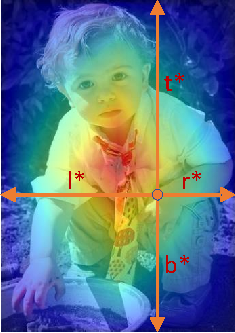
\includegraphics[width=0.2\linewidth]{figures/siamese_tracking/fcos_centerness.pdf}}
    \caption[Centerness visualization]{Red, blue, and other colors denote $1$, $0$ and the values between them, respectively. Centerness is calculated as given by \eqtext{}~\ref{eq:Centerness} and decays from $1$ to $0$ as the location deviates from the center of the object. Best viewed in color. \externalsrc{\cite{tian2019fcos}}}
    \label{fig:FCOSCenterness}
\end{figure}
% ------------------------------------------------------------------------------

% ##############################################################################
\subsection{Training and Inference Phases}

% ------------------------------------------------------------------------------
\begin{figure}[H]
    \centering
    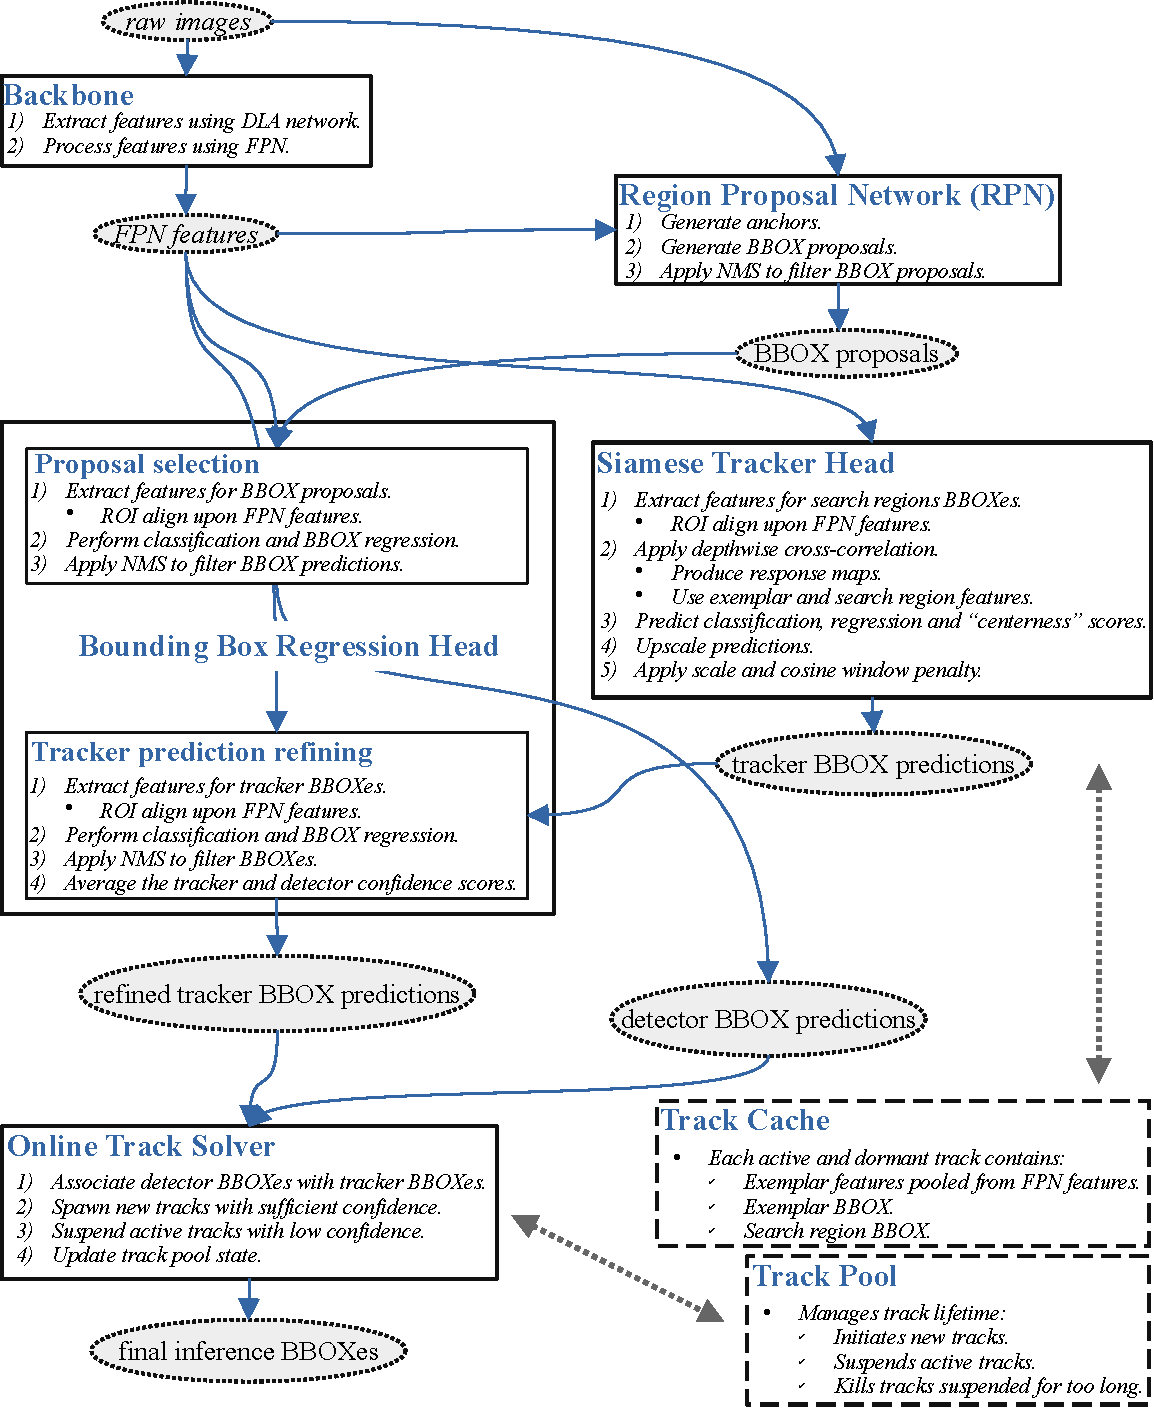
\includegraphics[width=\linewidth]{figures/siamese_tracking/siammot_inference_diagram.pdf}
    \caption[\gls{siammot} inference diagram]{The inference pipeline in the \gls{siammot} tracker. Backbone features that are a result of intricate \gls{dla} and \gls{fpn} processing are fed into the detector and the tracker. The predictions from the tracker are further refined using the detector head. The two heads function on top of backbone features through the lens of \gls{roi} align operations. During the inference, the ``online solver'' works only with the final \glspl{bbox} produced by the tracker and the detector. It utilizes a simple caching mechanism to store the features belonging to active or dormant objects. The decision-making regarding initialization, suspension, and complete removal of the track is performed within the ``track pool'' module.}
    \label{fig:SiamMOTInference}
\end{figure}
% ------------------------------------------------------------------------------

The \gls{siammot} model can be trained in an end-to-end fashion, which is one of its great advantages in terms of usability. The general loss function can be formulated as
\begin{equation}
    \label{eq:SiamMOTGeneralLoss}
    \lossf = l_{rpn} + l_{detect} + l_{motion},
\end{equation}
where the $l_{rpn}$ as well as the $l_{detect}$ are standard \gls{rpn}~\cite{ren2017fasterrcnn} and detection-subnetwork~\cite{girshick2015fast} losses, respectively. The $l_{motion}$ loss is used to train the Siamese tracker.

For better understanding, we suggest the reader follows the diagram in \figtext{}~\ref{fig:SiamMOTInference}. At inference, the well-established \gls{iou}-based \gls{nms} operation (\sectiontext{}~\ref{ssec:NonMaximumSuppression} on page \pageref{ssec:NonMaximumSuppression}) is exploited to process the outputs of the detection and tracker subnetwork independently. The subsequent phase aimed at spatial matching is used to merge detections with the tracker output. This stage also involves the already mentioned \gls{iou}-based \gls{nms} operation.

% ------------------------------------------------------------------------------
\begin{figure}[!t]
    \centering
    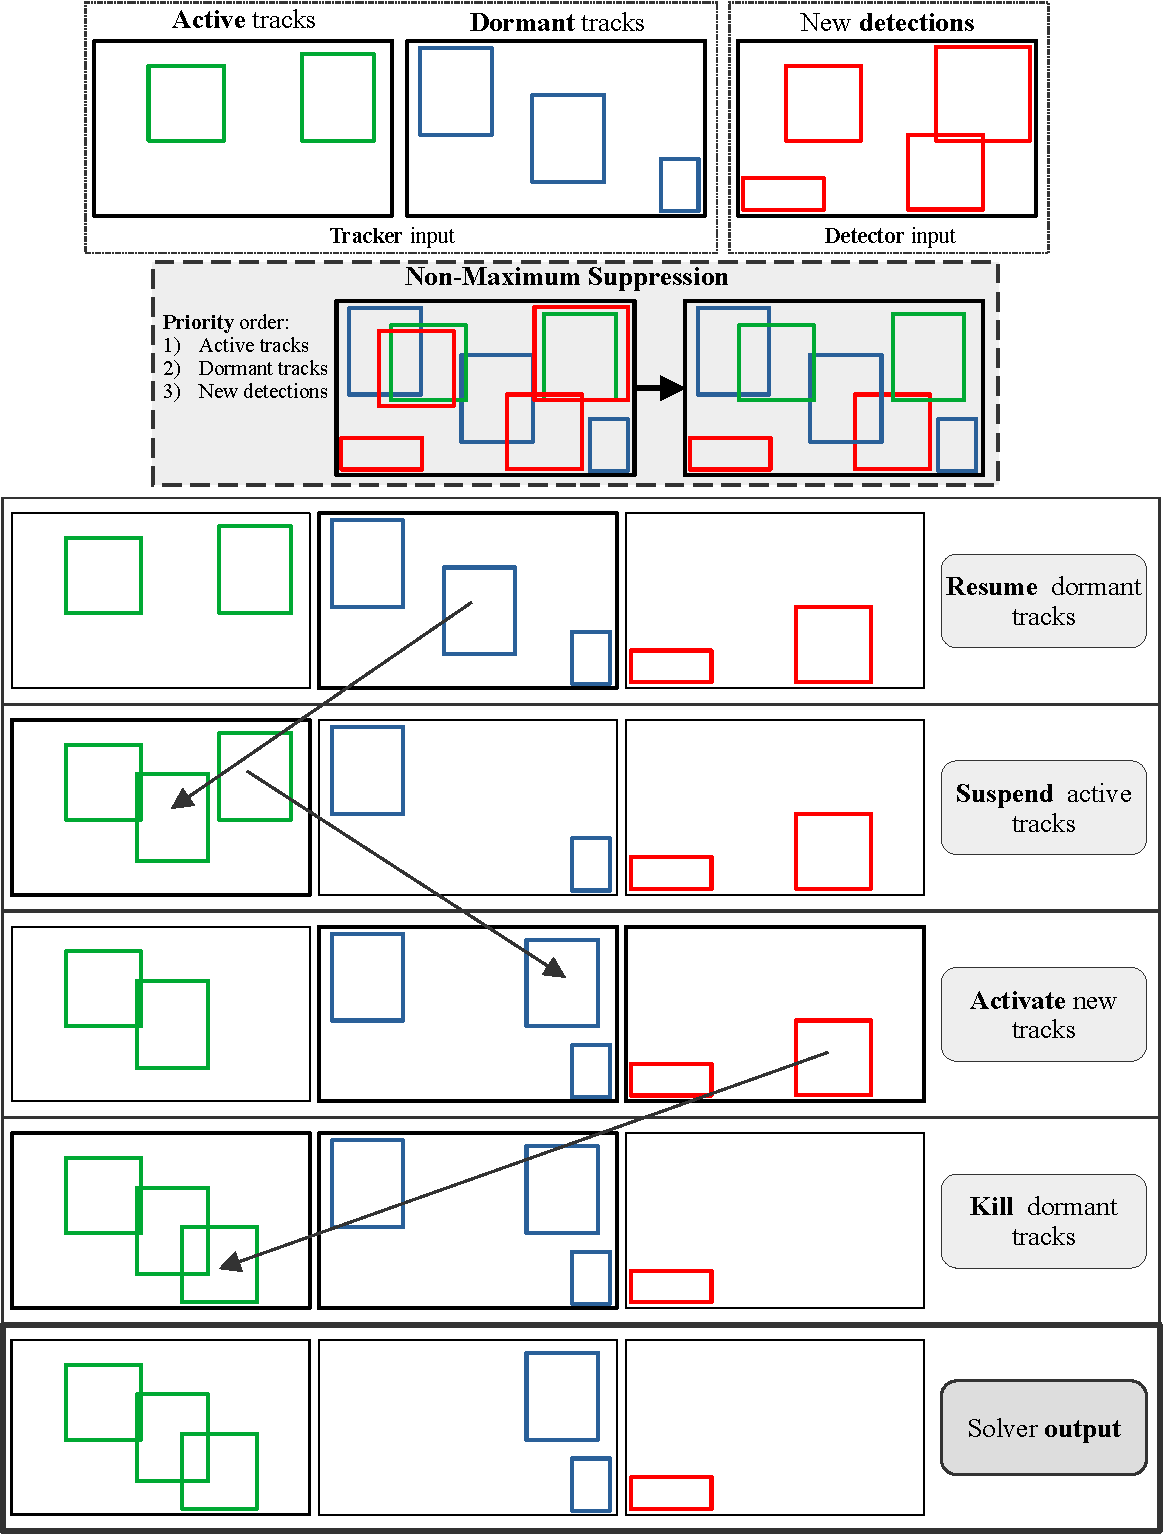
\includegraphics[width=0.85\linewidth]{figures/siamese_tracking/siammot_online_solver.pdf}
    \caption[\gls{siammot} online solver]{Here we present the process which the tracker, as well as the detector predictions for the current frame, undergo to derive the final tracker output. At first, all the \glspl{bbox} are merged upon which a \gls{nms} algorithm is performed. The \gls{nms} algorithm preserves the priority that active tracks are processed primarily, then followed by the dormant tracks. The remaining detections are filtered as last. The \gls{nms} algorithm does not have to be modified at all, since the priority can be induced by altering the associated score values. After the \gls{nms} stage, the dormant tracks with sufficient confidence are reactivated. Conversely, active tracks with low confidence are suspended. Then, if there are detections with high confidence, new tracks are established. The process finishes off by permanently killing dormant tracks that have lasted for more than some specific number of frames without instantiation. Note that even though the solver outputs instances of all three categories, only the active tracks are part of the inference.}
    \label{fig:SiamMOTOnlineSolver}
\end{figure}
% ------------------------------------------------------------------------------

The spatial matching and the object identity association happen within the non-trainable module that is activated only during the inference, further referred to as the \emph{online solver}. The purpose is to propagate existing object identities to the future frames given the predictions made by the object detector and object tracker independently. In \figtext{}~\ref{fig:SiamMOTOnlineSolver}, we provide a graphical illustration of the original algorithm. The solver algorithm is governed by the following rules listed below. Let $\subsup{v}{i}{t}$ be the visibility confidence, then
\begin{enumerate}
    \item the object's trajectory is continued as long as its visibility confidence is above a specific threshold $\alpha$, otherwise, this trajectory becomes dormant,
    \item a new trajectory is spawned in case there is a non-matched detection (during the spatial-matching process) and its visibility confidence is above a threshold $\beta$,
    \item a dormant trajectory is terminated, \ietext{}, the object ID will never be used again if its visibility confidence is below $\alpha$ for $\tau$ consecutive frames.
\end{enumerate}

This model tackles short-term occlusion. It is one of the key incentives that led us to consider this architecture for experiments, which is the model's ability to handle occlusion. In the beginning, we guessed that this phase could be improved upon due to its inherent simplicity. However, regardless of how rudimentary their approach may seem, it implicitly addresses plenty of frequent cases that appear in object tracking in a competent way. Our endeavors later described often involved a minor improvement in rare situations with simultaneous minor detriments to common situations. Therefore, the outcome of performing worse than the baseline on average was usually inescapable.

A short-term occlusion can be defined as having the visibility confidence for the currently tracked object below the threshold $\alpha$. In \gls{siammot}, instead of ceasing the track's existence, the relevant information is kept in memory and thus the search for the exemplar continues until $\tau > 1$ frames have been processed in hope of re-instantiating the object. The most recently predicted location and its corresponding feature frames extracted from the backbone are utilized as the searching template. As a side note, a very similar solver approach has also been adopted in numerous works, such as~\cite{bawley2016simple, wojke2017simple, zhou2020tracking, bergmann2019tracking}. In essence, it is simple yet very effective. As our experiments will later demonstrate, it is exceedingly difficult to surpass its performance in general by a significant margin.

% ##############################################################################
\subsection{Implementation Details}

\subsubsection{Pre-training}

Overall, the model is not difficult to train. By difficult training, we mainly mean instability and sensitivity to hyperparameters. However, the training itself requires a great deal of GPU VRAM available to use sufficiently large minibatches. As far as our development experience with the \gls{siammot} model is concerned, we used the \texttt{NVidia}~\cite{webnvidia} \texttt{RTX 2080Ti} graphics cards which provides $4352$ CUDA cores together with $11$GB of GDDR6 memory. For training, we often exploited an existing backbone model pre-trained on ImageNet~\cite{deng2009imagenet} dataset provided by the original authors. Even though there is the entire model available pre-trained on \mscoco{}~\cite{lin2014mscoco} dataset, we decided to avoid it due to the conflicting nature of object classes. We observed better performance when training vehicle detection from scratch rather than trying to ``re-wire'' the model to dismiss detecting objects we wanted to avoid in the first place, \egtext{}, pedestrians.

\subsubsection{Gradient Accumulation}

As the majority of our experiments involved expanding the model by adding additional heads, we often struggled with the amount of available GPU VRAM to preserve a reasonable size of minibatches. To this end, we experimented with gradient accumulation, which allows the user to postpone the model weight updating after more minibatches have been processed (\figtext{}~\ref{fig:GradientAccumulation}). Therefore, the programmer may simulate using larger minibatches than are actually utilized. We emphasize the importance of not updating the model variables must during the accumulation phase so as to ensure that all the mini-batches are processed by the same model to calculate their gradients. Only after accumulating the gradients of the values of the model weights can be adjusted accordingly.

For a brief illustration, let $w$ be a single weight we want to update with respect to the computed gradient using the loss function $f$. Our goal is to adjust the weight at time $t$ and thus produce the weight at time $t + 1$. The learning rate is denoted by $\alpha$. So, the gradient update is usually performed as
\begin{equation}
    w^{t + 1} = w^t - \alpha \nabla \func{f}{w^t}.
\end{equation}
When using gradient accumulation, the update step is modified as
\begin{equation}
    w^{t + 1} = w^t - \alpha \sum_{i = 1}^{n} \nabla \func{f}{w^t}_i,
\end{equation}
where $n$ is the number of accumulated minibatches.

% ------------------------------------------------------------------------------
\begin{figure}[!t]
    \centering
    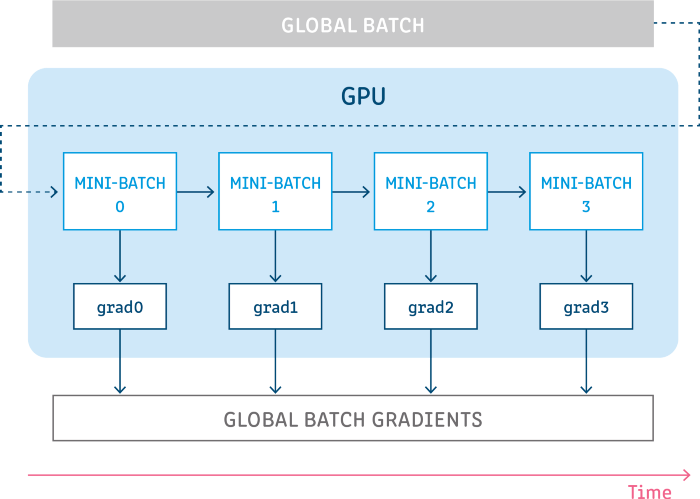
\includegraphics[width=0.6\linewidth]{figures/siamese_tracking/gradient_accumulation.png}
    \caption[Gradient accumulation]{Gradient accumulation is a mechanism that allows splitting the minibatch of samples — used for training a neural network — into several even smaller mini-batches of samples that will be processed sequentially. \externalsrc{\cite{webgradaccumulation}}}
    \label{fig:GradientAccumulation}
\end{figure}
% ------------------------------------------------------------------------------

Considering the advantages outlined above, it is necessary to acknowledge the potential drawbacks. For example, if batch normalization~\cite{ioffe2015batchnorm} layers are used within the model, then the use of gradient accumulation may have a detrimental effect upon their performance. The reason is that batch normalization layers compute the statistics with respect to a single minibatch. These layers, in their standard formulation and commonly adopted implementation, are incapable of accomodating their inner workings to adequately administer multiple sequential minibatches. However, there is ongoing research in the direction of group normalization as well, namely the works~\cite{wu2018groupnorm}~and~\cite{zhou2020batchgroupnorm}.
